%%%%%%%%%%%%%%%%%%%%%%%%%%%%%%%%%%%%%%%%%%%%%%%%%%%%%%%
%% QUESTIONS FOR MATH 4MB/6MB ASSIGNMENT 4.          %%
%% The question texts are used in several documents: %%
%% assignment, solutions, template,                  %%
%% hence it is better to load them from this file.   %%
%%%%%%%%%%%%%%%%%%%%%%%%%%%%%%%%%%%%%%%%%%%%%%%%%%%%%%%

\newcommand{\TSa}{%
You should have received the following data files by e-mail:
\begin{center}
\tt
meas\_uk\_\_lon\_1944-94\_wk.csv\\
meas\_uk\_\_lpl\_1944-94\_wk.csv
\end{center}
These plain text comma-separated-value files list weekly cases of measles (in London and Liverpool, England, from 1944 to 1994).  Depending on which research direction you select, you might receive other files in the same \code{ymdc} (year,month,day,count) format, where the count column might contain cases or deaths, for example.  Write the following \Rlogo functions:
}

\newcommand{\TSai}{%
\magcode{read.ymdc()}.  Read a file in \code{ymdc} format and return a data frame containing these data and including a \code{date} column that has \Rlogo's \magcode{Date} class.  The first (and potentially only) argument to this function should be the \code{filename} of the data file to be read.
}  

\newcommand{\TSaii}{%
\magcode{time.plot()}.  Given a data frame produced using \magcode{read.ymdc()}, display the associated time plot.  The first argument of the function should be the data frame.  Further optional argument(s) should allow the user to smooth the time series with a moving average.  By default, this function should create a new plot but there should be an option to add to an existing plot. Implement this by having a logical \code{add} argument that is false by default (\code{add=FALSE}).  This will allow you to add a smoothed version of the time series on top of the raw data, for example.  The final argument should be the ellipsis (\code{\dots}) so that details such as colour and line style can be passed to the plotting commands used in this function.
}

\newcommand{\TSaiii}{%
\magcode{periodogram()}.  Given a data frame produced using \magcode{read.ymdc()}, display the associated \emph{period   periodogram} (power spectrum as a function of period).  The first argument of the function should be the data frame.  By default, the entire time series should be used, but optional argument(s) should allow the user to specify a time range of interest.  Use \Rlogo's \magcode{spectrum()} function to compute the power spectrum.  Have \code{add} and \code{\dots} arguments as in \magcode{time.plot()}. Note that if \code{v} is a vector containing a time series of interest, you can obtain and plot its \emph{frequency} periodogram as follows.
}

\newcommand{\TSb}{%
Using your functions, make a multi-panel plot that clearly shows the temporal pattern of the time series and how its frequency structure changes over time.  Think carefully about how to make this multi-panel figure as clear as possible for yourselves and your readers.  Describe your figure, explaining what aspects of your figure you feel are puzzling or interesting and may be possible to understand using mechanistic mathematical modelling.  (Repeat this for each of the epidemic time series you are given.)
}

\newcommand{\SEintro}{%
Consider the SI model,
%
\begin{equation}\label{E:SI}
  \frac{dI}{dt} = \beta (N-I) I \,, \qquad I(0)=I_0,
\end{equation}
%
where $\beta$ is the transmission rate, $N$ is the population size and $I(t)$ is the number of infected individuals at time $t$.
}

\newcommand{\SEa}{%
Write an \Rlogo function \magcode{SI.Gillespie()} that uses the Gillespie algorithm to produce a realization of a stochastic process whose mean field dynamics are given by equation \eqref{E:SI} in the limit $N\to\infty$.  Your function should have arguments \code{beta}, \code{N}, \code{I0} and \code{tmax} (the time at which to end the simulation).  You may find it helpful (conceptually) to write equation~\eqref{E:SI} in two-variable form:
  \begin{subequations}
    \begin{align}
      \frac{dS}{dt} &= -\beta S I \,, \qquad S(0)=N-I_0, \\
      \frac{dI}{dt} &= \beta S I \,, \qquad\quad I(0)=I_0.
    \end{align}
  \end{subequations}
Note that there is only one type of event that can occur, so the second part of the Gillespie algorithm (what type of event occurred) is trivial for this model.
}

\long\def\SEb{%
Make a multi-panel plot comparing the deterministic and stochastic dynamics of the SI model for $\beta=1$, $I_0=1$ and $N\in\{32,10^2,10^3,10^4\}$ ($N=32$ is close to $10^{1.5}$).  Each panel should correspond to a different value of $N$ and should show 30 stochastic realizations together with the deterministic solution.

\emph{\underline{Note}:} To make stochastic simulations exactly reproducible use \texttt{\color{magenta}set.seed()}.
}

\newcommand{\Rintro}{%
The natural history of smallpox is shown in \fref{smpxnathist}.  The US Centers for Disease Control and Prevention (CDC) has recently discovered that a group of bioterrorists plans to reintroduce smallpox to the United States.  The CDC has reason to believe that the terrorists are also bioengineers and have successfully altered the virus so that it causes the early rash stage to be twice as long as it was when the virus was last circulating naturally in the 1970s.  Moreover, the existing smallpox vaccine apparently provides no protection against the altered virus.  The CDC wants your opinion on how the alterations to the virus will affect $\R_0$ and the expected final size of an epidemic if the planned attack is successful.
}

\newcommand{\Ra}{%
Construct a compartmental (ODE) smallpox transmission model based on the natural history specified in \fref{smpxnathist}, including vital dynamics but ignoring disease-induced death.
}

\newcommand{\Rb}{%
Use a biological argument to find a formula for $\R_0$.
}

\newcommand{\Rc}{%
Calculate $\R_0$ using the next generation matrix approach.  \emph{\underline{Note}:} Your solution should include $\mathcal F$, $\mathcal V$, $F$, $V$, and $FV^{-1}$, in the most human-friendly form you can find.  However, feel free to use symbolic manipulation software such as \texttt{Maple}, {\slshape Mathematica\/} or \href{http://www.sagemath.org/}{sage} to help with the necessary algebra and matrix computations.
}

\newcommand{\Rd}{%
Based on your model, and $\R_0\sim5$ for unaltered smallpox, what can you say about the difference in $\R_0$ that can be expected for the newly engineered virus vs.\ the original virus?  
    %% (\emph{\underline{Note}:} If you make use of other sources of information, such as books or web sites, cite them appropriately.)
}

\newcommand{\qRe}{% \Re is TeX's real part symbol so can't use it
Write a paragraph that you can imagine e-mailing to the CDC, in which you do your best to answer their questions.
    %% It would be good to get them to find a formula for the growth
    %% rate and then explain how to use their model to estimate R0 for
    %% the new virus after the growth rate has been measured
    %% empirically.  But, the growth rate cannot be found analytically
    %% (the characteristic polynomial has degree 5) so the problem
    %% becomes longer than I want to burden them with right now.
}

\newcommand{\smpxnathistfig}{%
%
\begin{figure}[h]
\begin{center}
\scalebox{1}{
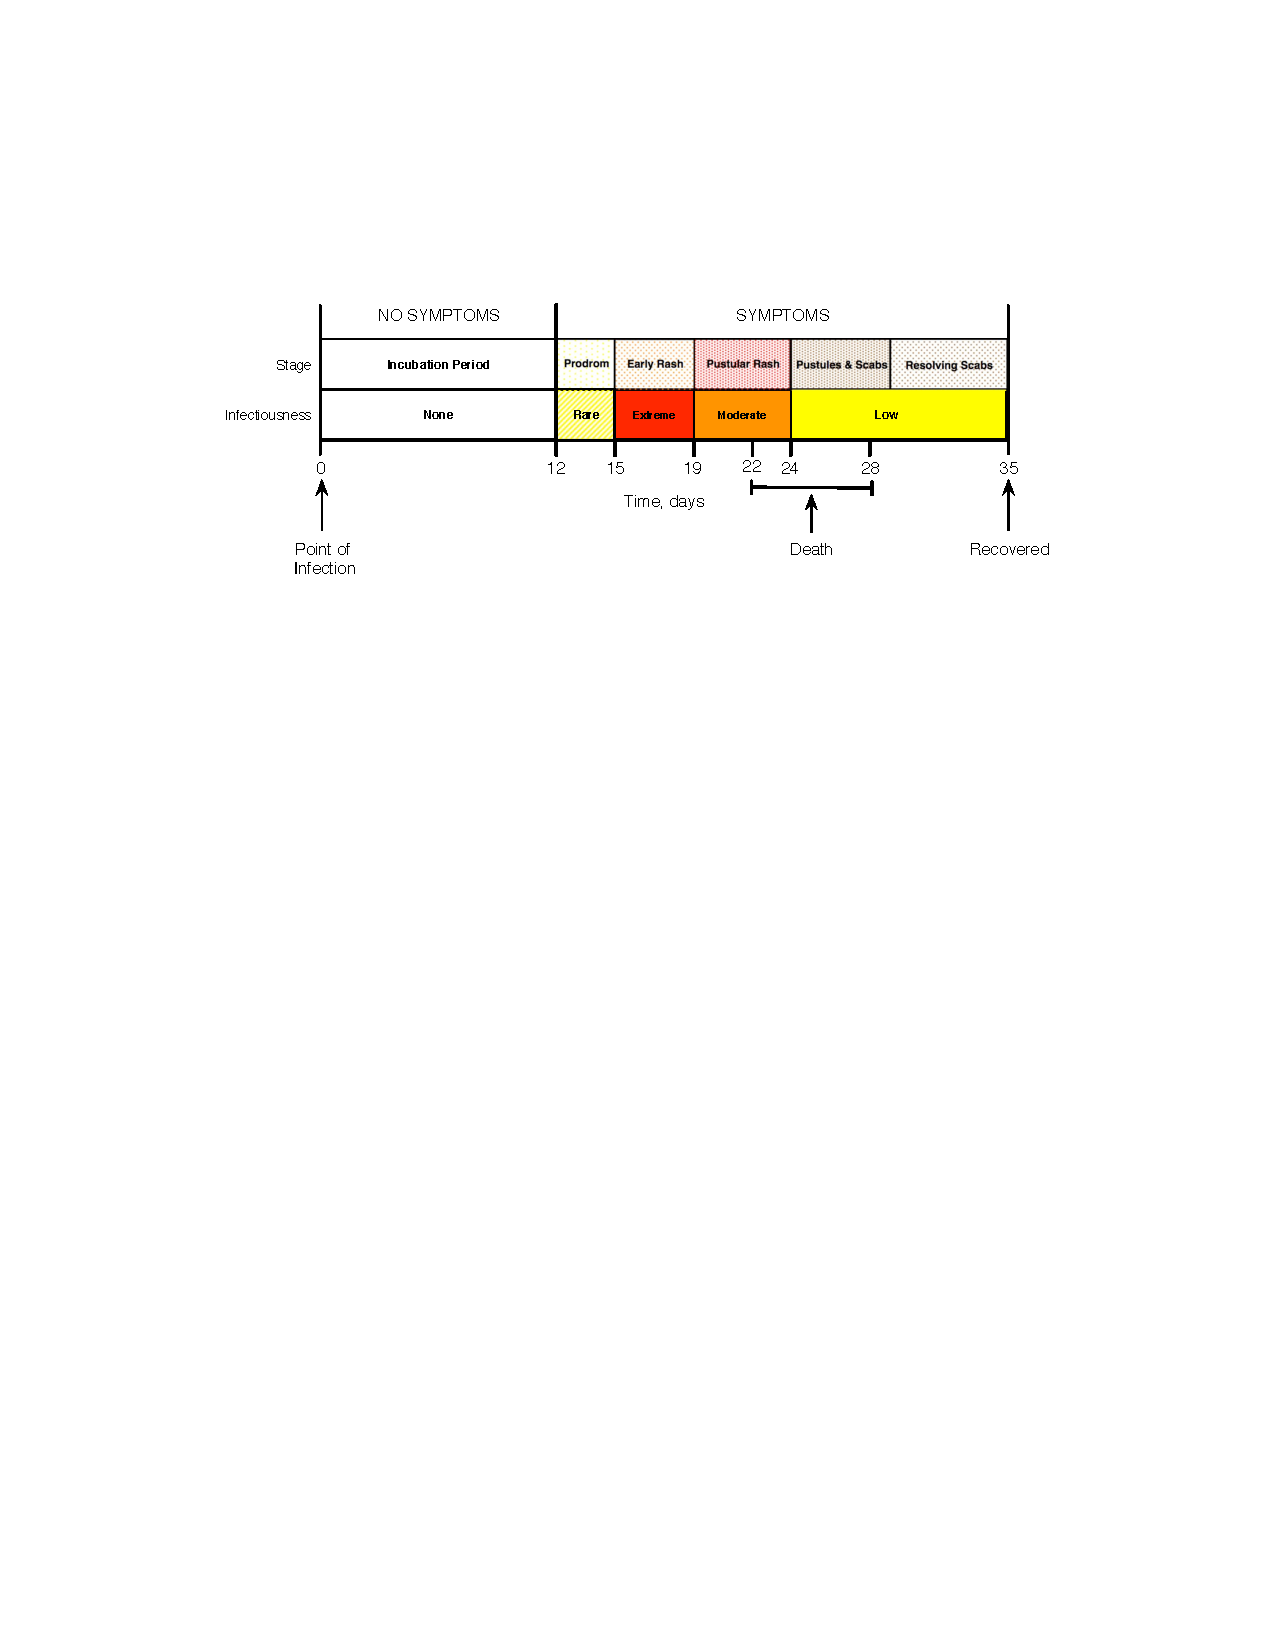
\includegraphics{smpxnathist_p82.pdf}
}
\end{center}
\caption{The natural history of smallpox infection. The prodrom stage begins with fever but the patient is very rarely contagious. Early rash is the most contagious stage, when the rash develops and transforms into bumps. During the pustular rash stage bumps become pustules, which then turn into scabs during the pustules and scabs stage and fall off during the resolving scabs stage. The infected person is contagious until the last scab falls off.  (\emph{This is Figure 3.4 from page 82 of Olga Krylova's 2011 McMaster University PhD thesis.})}
\label{F:smpxnathist}
\end{figure}
%
}

%%\bibliographystyle{vancouver}
%%\bibliography{4mba4_2018}
